


\newpage
\section*{Problem Defintion}
\subsection*{Domain}
The computational domain resembles the classic cfd benchmark with an added bar, with dimensions: \\
The box: L = 2.5, H = 0.41 \\
The bar: l = 0.35, h = 0.02 \\
The circle is positioned at (0.2, 0.2) making it 0.05 of center from bottom to top, this is done to induce oscillations to an otherwise laminar flow.\\
Boundary conditions:\\
The fluid velocity has a parabolic profile on the inlet that changes over time:\\

\begin{align*}
u(0,y) &= 1.5u_0 \frac{y(H-y)}{(\frac{H}{2})^2}  \\
u(0,y,t) &= u(0,y)\frac{1-cos(\frac{\pi}{2}t)}{2} \text{  for  } t<2.0 \\
u(0,y,t) &= u(0,y) \text{  for  } t \leq 2.0
\end{align*}

We set no slip on the "floor" and "ceiling" so to speak.\\
On the fluid solid interface the boundary conditions are set to:
$$  \sigma_f n_f = \sigma_s n_s \hspace{4mm} on  \hspace{2mm}\Gamma^0 (interface)   $$
In our variational form we leave this out and so implying that they are equal.

\subsection*{CSM test}
Parameters
\begin{table}[h]
\centering
\caption{My caption}
\label{my-label}
\begin{tabular}{|l|l|l|l|}
\hline
Parameters & CSM1 & CSM2 & CSM3 \\ \hline
$\rho_f[10^3 \frac{kg}{m^3}]$ & 1 & 1 & 1 \\ \hline
$\nu_f [10^{-3} \frac{m^2}{s}]$ & 1 & 1 & 1 \\ \hline
$u_0$ & 0 & 0 & 0 \\ \hline
$\rho_s[10^3 \frac{kg}{m^3}]$ & 1 & 1 & 1 \\ \hline
$\nu_s$ & 0.4 & 0.4 & 0.4 \\ \hline
$\mu_s[10^6 \frac{m^2}{s}]$ & 0.5 & 2.0 & 0.5 \\ \hline
$g $ & 2 & 2 & 2 \\ \hline
\end{tabular}
\end{table}

\begin{table}[h!]
\centering
\caption{CSM 1}
\label{my-label}
\begin{tabular}{|l|l|l|l|}
\hline
elements & dofs & ux $[10^{?3}]$ & uy $[10^{?3}]$ \\ \hline
725 & 1756 & -5.80951654915 & -59.4781430115 \\ \hline
2900 & 6408 & -6.77960453995 & -64.2130757639 \\ \hline
11600 & 24412 & -7.08597041285 & -65.635825349 \\ \hline
46400 & 95220 & -7.11626976966 & -65.7456687273 \\ \hline
ref & ref & -7.187 & -66.10 \\ \hline
\end{tabular}
\end{table}

% Please add the following required packages to your document preamble:
% \usepackage{booktabs}
\begin{table}[]
\centering
\caption{CSM 2}
\label{my-label}
\begin{tabular}{@{}|l|l|l|l|@{}}
\hline
Elements & Dofs & ux $[10^{-3}] $& ux $[10^{-3}] $\\ \hline
725 &  1756 & -0.375962146908 & -15.1950342598 \\ \hline
2900 & 6408 & -0.441308781709 & -16.4643196042\\ \hline
11600 & 24412 & -0.462087305294 & -16.8478689583 \\ \hline
46400 & 95220 & -0.464128022327 & -16.8782135872\\ \hline
ref & ref & -0.4690 & -16.97 \\ \hline
\end{tabular}
\end{table}


\begin{figure}[ht] 
  \begin{subfigure}[b]{0.5\linewidth}
    \centering
    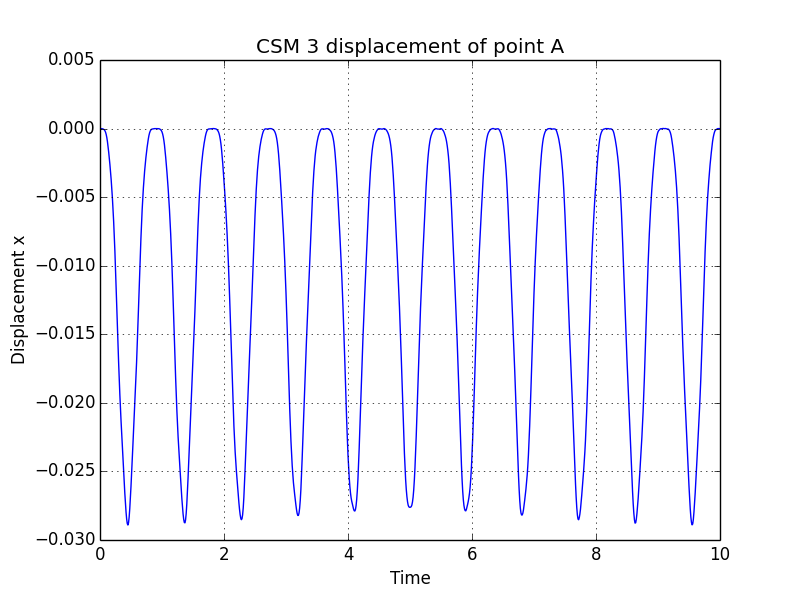
\includegraphics[width=0.75\linewidth]{./Verification_Validation//Hron_Turek/dis_x.png} 
    \caption{Displacement in x-direction} 
    \label{fig7:a} 
    \vspace{4ex}
  \end{subfigure}%% 
  \begin{subfigure}[b]{0.5\linewidth}
    \centering
    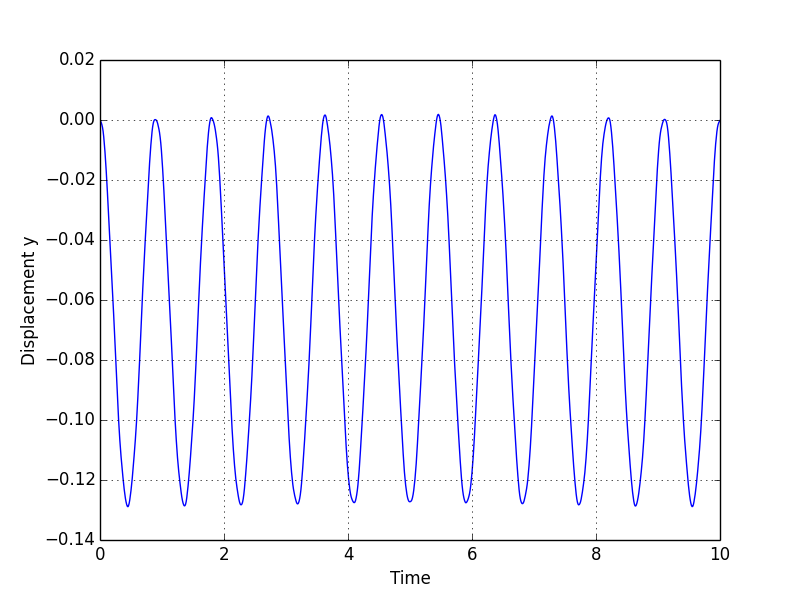
\includegraphics[width=0.75\linewidth]{./Verification_Validation//Hron_Turek/dis_y.png} 
    \caption{Displacement in x-direction} 
    \label{fig7:b} 
    \vspace{4ex}
  \end{subfigure} 
  \begin{subfigure}[b]{0.5\linewidth}
    \centering
    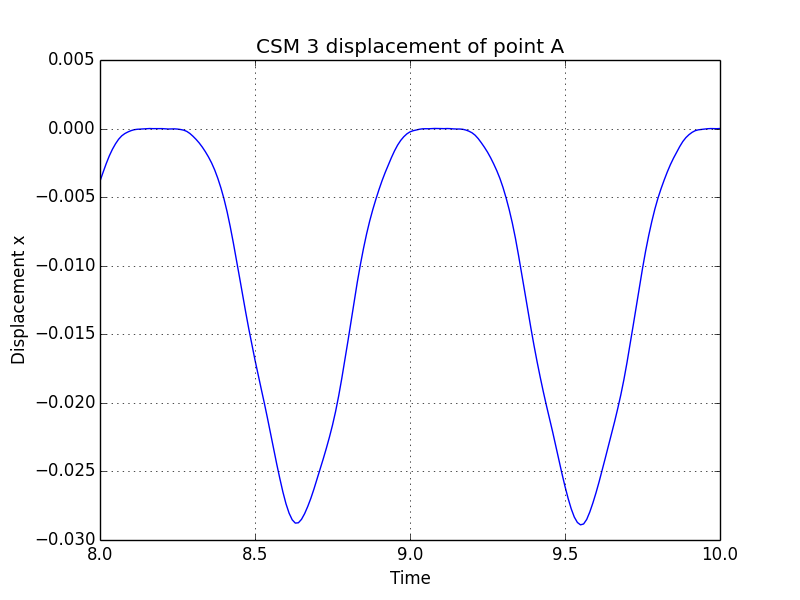
\includegraphics[width=0.75\linewidth]{./Verification_Validation//Hron_Turek/dis_x_short.png} 
    \caption{Displacement in x-direction} 
    \label{fig7:c} 
  \end{subfigure}%%
  \begin{subfigure}[b]{0.5\linewidth}
    \centering
    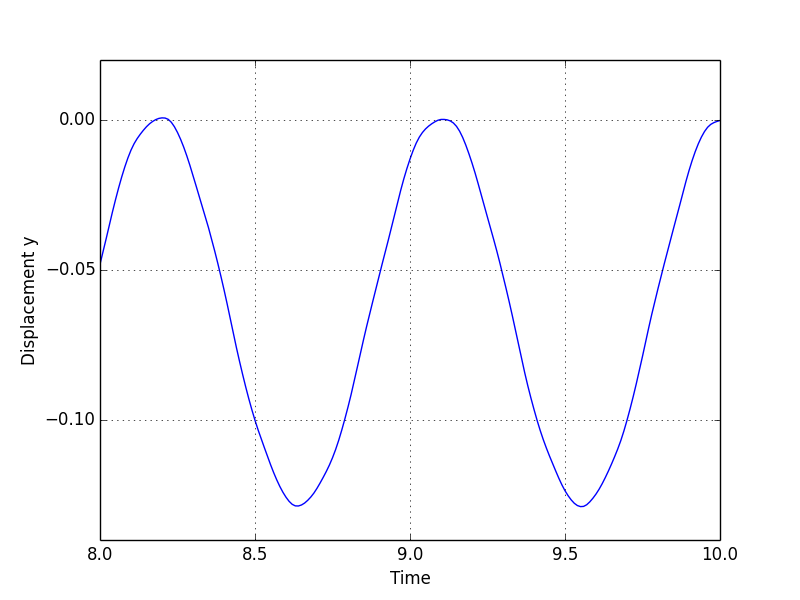
\includegraphics[width=0.75\linewidth]{./Verification_Validation/Hron_Turek/dis_y_short.png} 
    \caption{Displacement in x-direction} 
    \label{fig7:d} 
  \end{subfigure} 
  \caption{Displacement of point A}
  \label{fig7} 
\end{figure}



\newpage 

\subsection*{FSI test}
\begin{table}[ht]
\centering
\caption{Parameters}
\label{my-label}
\begin{tabular}{|l|l|l|l|}
\hline
Parameters & FSI1 & FSI2 & FSI3 \\ \hline
$\rho_f[10^3 \frac{kg}{m^3}]$ & 1 & 1 & 1 \\ \hline
$\nu_f [10^{-3} \frac{m^2}{s}]$ & 1 & 1 & 1 \\ \hline
$u_0$ & 0.2 & 1 & 2 \\ \hline
Re = $\frac{U d}{\nu_f}$ & 20 & 100 & 200 \\ \hline
$\rho_s[10^3 \frac{kg}{m^3}]$ & 1 & 10 & 1 \\ \hline
$\nu_s$ & 0.4 & 0.4 & 0.4 \\ \hline
$\mu_s[10^6 \frac{m^2}{s}]$ & 0.5 & 0.5 & 2 \\ \hline
\end{tabular}
\end{table}
Results: 
\begin{table}[h]
\centering
\caption{FSI 1}
\label{my-label}
\begin{tabular}{|l|l|l|l|l|l|l|}
\hline
Cells & Dofs & ux of A $[x10^{-3}]$ & uy of A $[x10^{-3}]$ & Drag & Lift & Spaces \\ \hline
2698 & 7095 & 0.0234594 & 0.797218  & 14.4963 & 0.915801 & P1-P1-P1 stab= 0.01 \\ \hline
2698 & 23563 & 0.02271 & 0.80288 & 14.1736 & 0.787891 & P2-P2-P1 \\ \hline
2698 & 23563 & 0.00581116 & 0.000000738678  & 12.07 & 0.02345 & P2-P2-P1 without weighting \\ \hline
10792 & 92992 & 0.0227341 & 0.808792 & 14.1855 & 0.801044 & P2-P2-P1 \\ \hline
43168 & 369448 & 0.227352 & 0.812595 & 14.227 & 0.797242 & P2-P2-P1 \\ \hline
\textbf{ref} & \textbf{ref} & \textbf{0.0227} & \textbf{0.8209} & \textbf{14.295} & \textbf{0.7638} & \textbf{ref} \\ \hline
\end{tabular}
\end{table}
In my monolithic 



